%This is the base for the certificat of the chatoische catalysator stipendien

\documentclass{article}
\title{Chaotisches Catalysator Stipendium}
%\date{2022/2023}
%\name{Mars Mustermensch}

%Packages used:
\usepackage{graphicx}
\usepackage[T1]{fontenc}
\usepackage{fontspec} % used to set custom font
\usepackage[a4paper, margin=0.5cm]{geometry}
\usepackage[document]{ragged2e}
\usepackage{changepage}
\usepackage{tikz} %used to place text over images
\usepackage{subfig}

%removes page number
\pagenumbering{gobble}

% Setting font sizes:
\newcommand{\smallfont}[1]{{%
  \fontsize{13pt}{15pt}\normalfont #1%
}}
\newcommand{\normfont}[1]{{%
  \fontsize{20pt}{24pt}\normalfont #1%
}}
\newcommand{\bigfont}[1]{{%
  \fontsize{30pt}{36pt}\normalfont #1%
}}

% Setting custom fonts:
\newfontfamily{\firasans}
  [Ligatures=TeX, % recommended
   UprightFont={*-Light},
   ItalicFont={*-Italic},
   BoldFont={*-Medium}]
  {FiraSans}
\newfontfamily{\monomaniac}
  [Ligatures=TeX, % recommended
  ]
  {MonomaniacOne-Regular.ttf}

%--------------------------------------------------------------------------------------------

\begin{document}

\begin{tikzpicture}
    \draw (0, 0) node[inner sep=0] {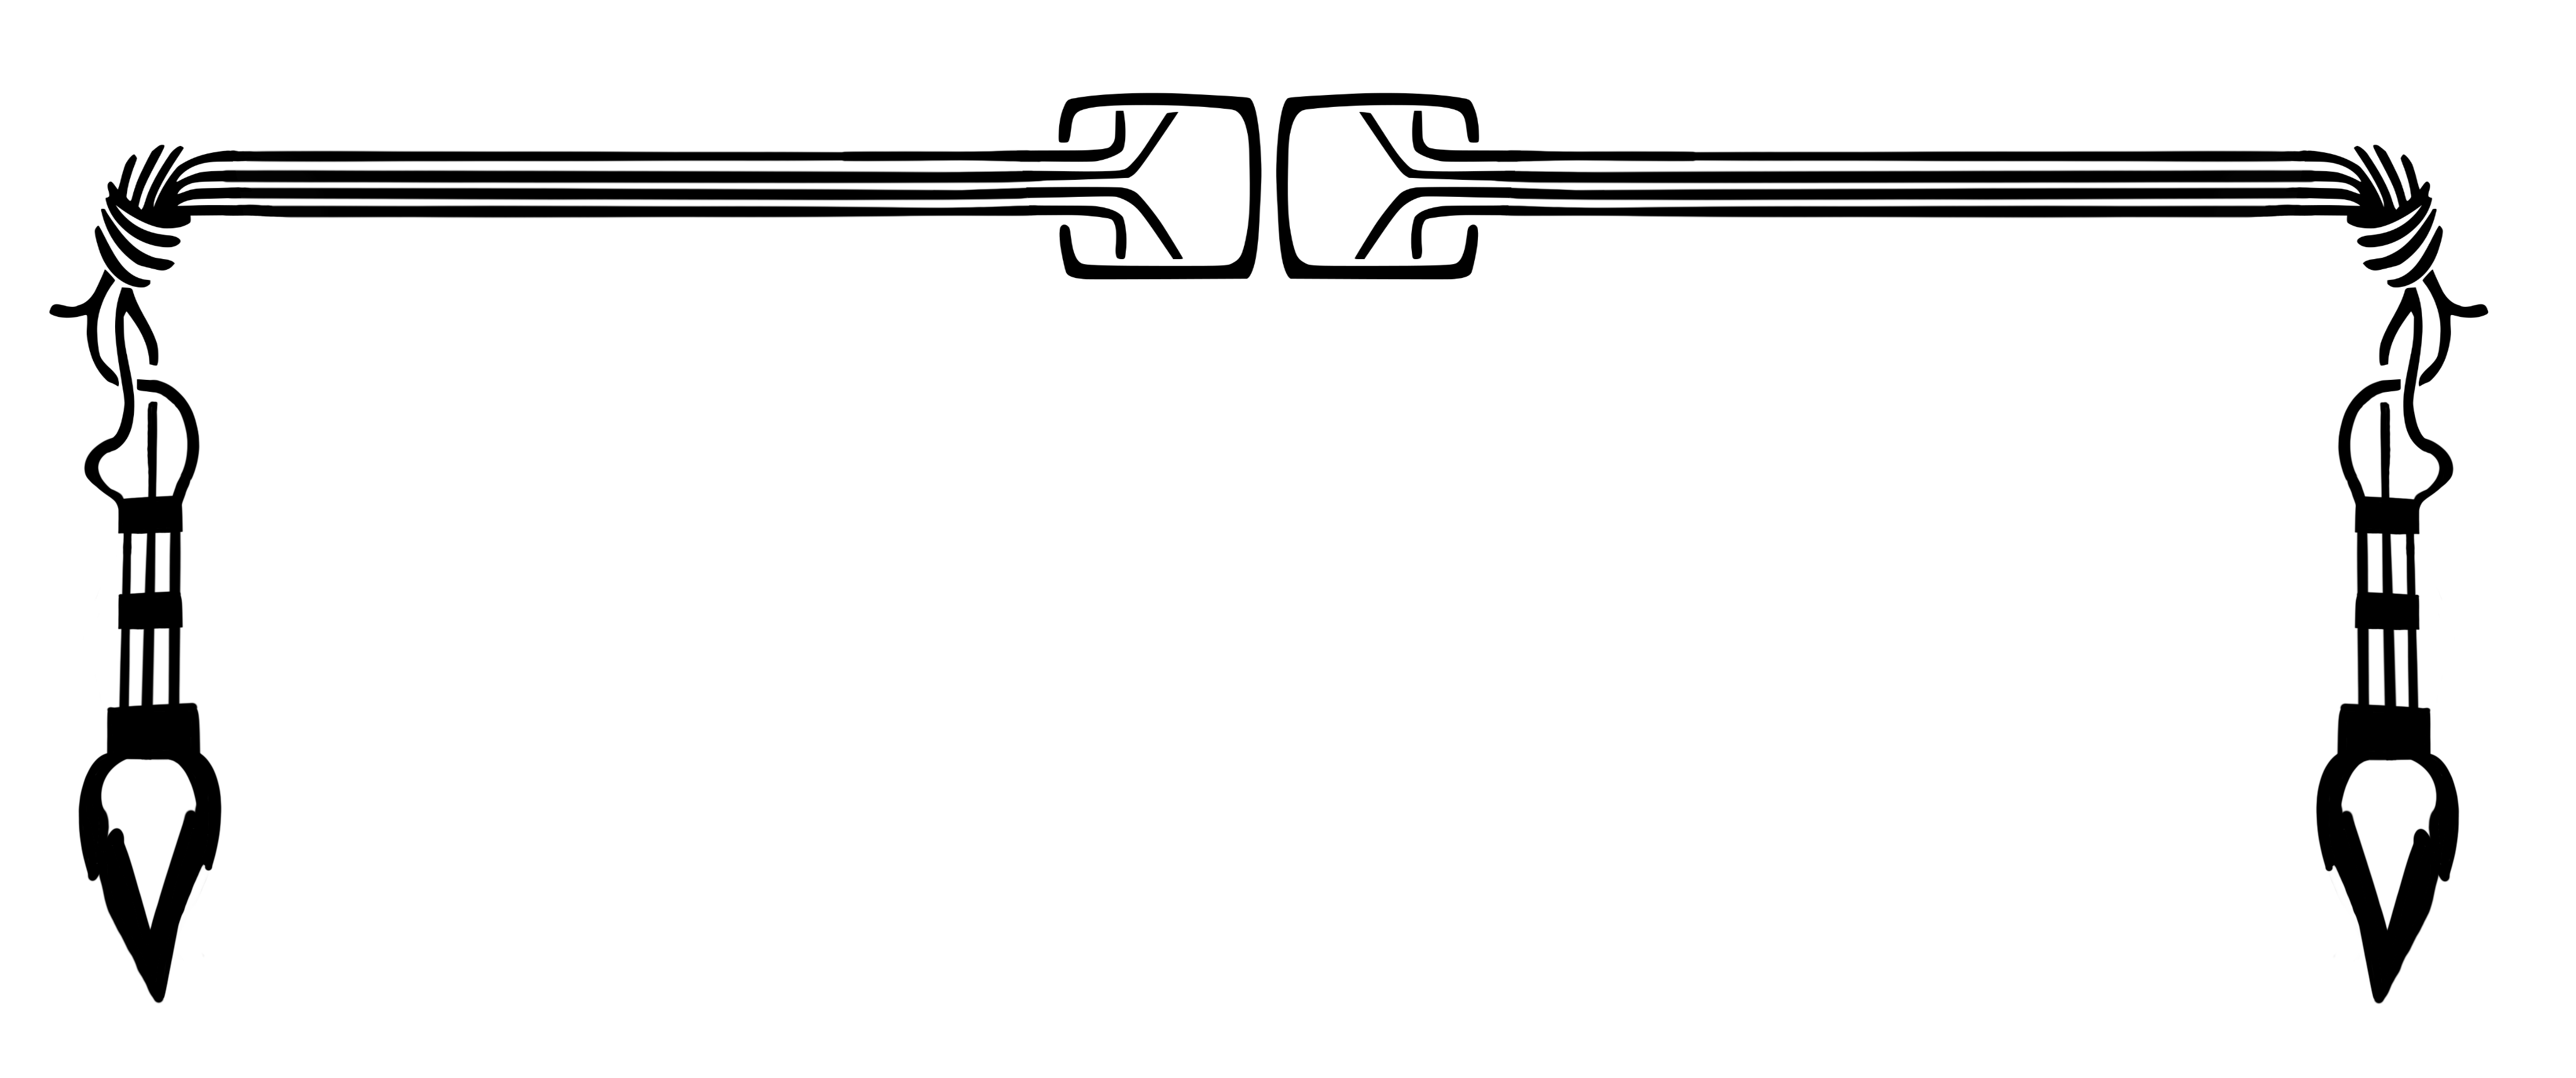
\includegraphics[width=0.95\paperwidth]{header}};
    \draw (0, 0) node {\normfont{\monomaniac 2023}};
    \draw (0, -1) node {\bigfont{\monomaniac Chaotisches Catalysator}};
    \draw (0, -2) node {\bigfont{\monomaniac Stipendium}};
    \draw (0, -3) node {\normfont{\monomaniac - Mars Mustermensch -}};
\end{tikzpicture}

\vspace{2cm}

\begin{adjustwidth}{3cm}{3cm}
    \smallfont{\firasans \RaggedRight Herzlichen Glückwunsch! \\ \smallskip
    Du hast uns mit deinem Thema überzeugt. Wir glauben dass nicht nur Computer das Leben zum Besseren verändern können, sondern auch deine Masterarbeit einen Mehrwert in dieser Gesellschaft schaffen wird. \\
    Der Chaos Computer Club e.V. fördert dich daher mit dem \\ Chaotischen Catalysator Stipendium in Höhe von 1.500€. \\[4\baselineskip]
    \par}
\end{adjustwidth}

\begin{adjustwidth}{3cm}{3cm}
    \RaggedLeft ---------------------------------------- \\
    \smallfont{\firasans Samuel Brinkmann}
\end{adjustwidth}

\begin{figure}[b]
	\begin{center}
		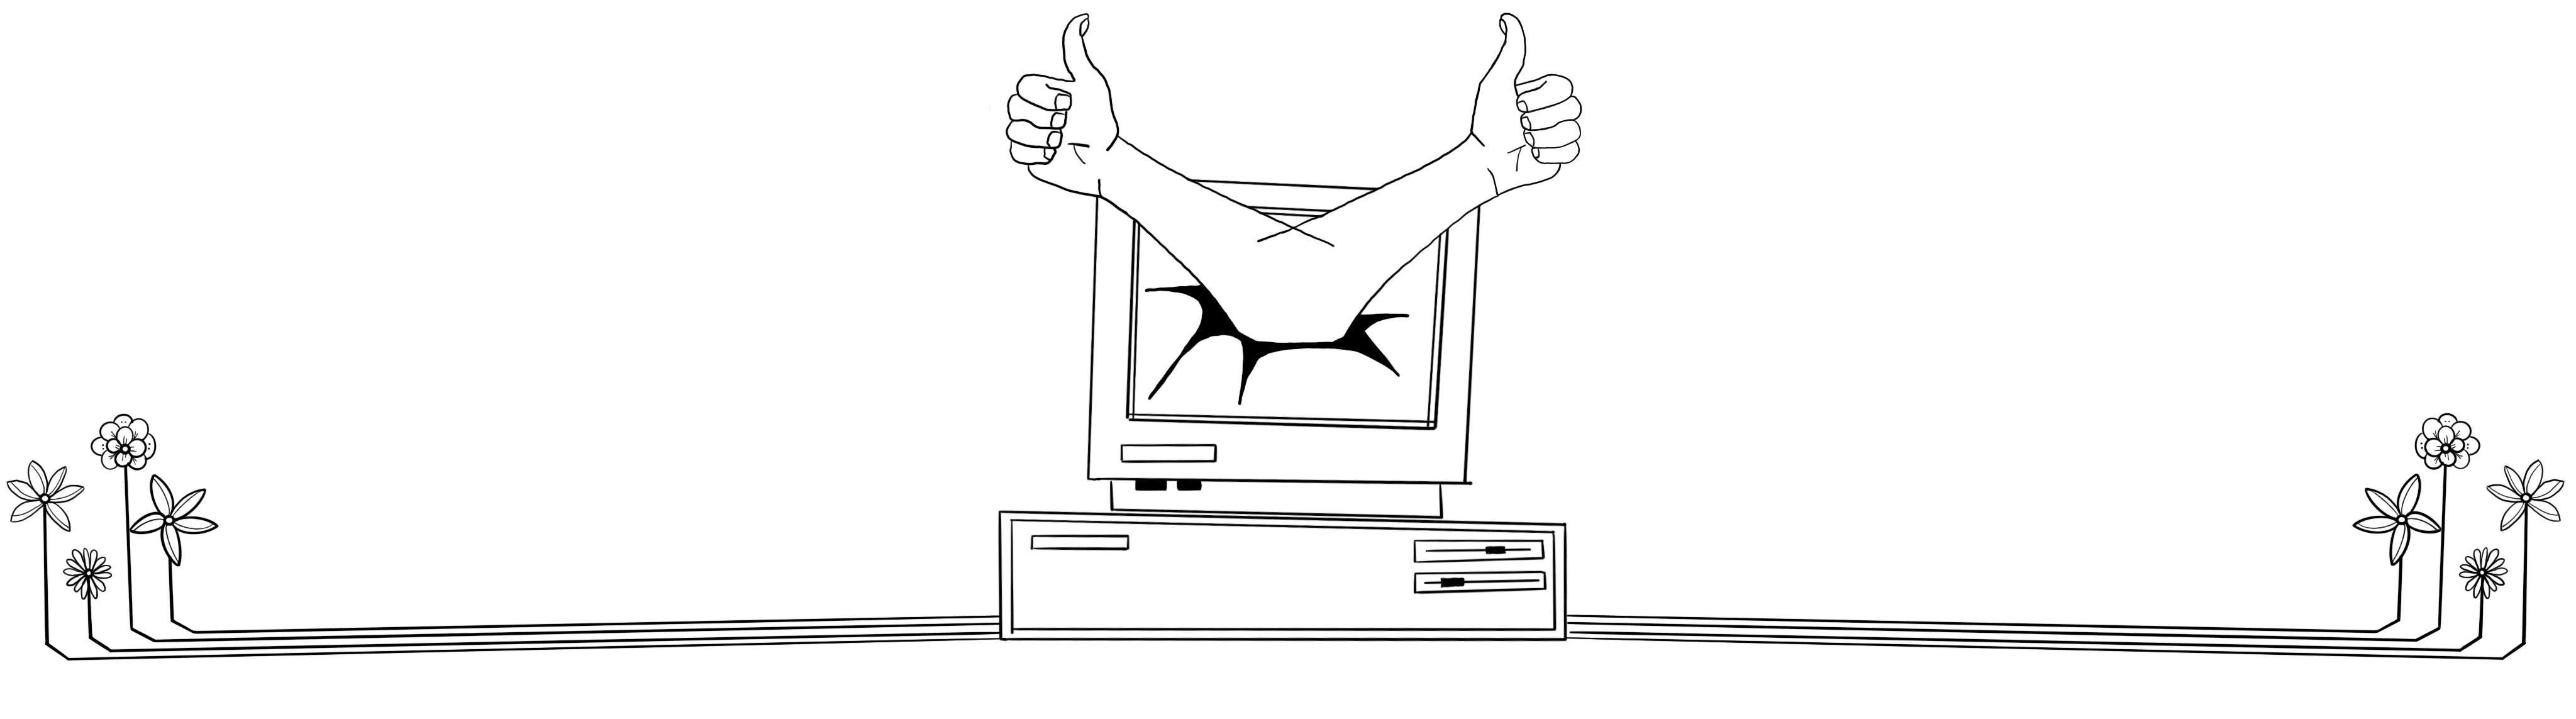
\includegraphics[width=0.9\paperwidth] {bottom-decoration}
	\end{center}
\end{figure}

\end{document}
